%
% Niniejszy plik stanowi przykład formatowania pracy magisterskiej na
% Wydziale MIM UW.  Szkielet użytych poleceń można wykorzystywać do
% woli, np. formatujac wlasna prace.
%
% Zawartosc merytoryczna stanowi oryginalnosiagniecie
% naukowosciowe Marcina Wolinskiego.  Wszelkie prawa zastrzeżone.
%
% Copyright (c) 2001 by Marcin Woliński <M.Wolinski@gust.org.pl>
% Poprawki spowodowane zmianami przepisów - Marcin Szczuka, 1.10.2004
% Poprawki spowodowane zmianami przepisow i ujednolicenie 
% - Seweryn Karłowicz, 05.05.2006
% Dodanie wielu autorów i tłumaczenia na angielski - Kuba Pochrybniak, 29.11.2016

% dodaj opcję [licencjacka] dla pracy licencjackiej
% dodaj opcję [en] dla wersji angielskiej (mogą być obie: [licencjacka,en])

\documentclass[en]{pracamgr}

\usepackage{amsmath}
\usepackage{amsfonts} 


%% Imports the package natbib
\usepackage[square,numbers]{natbib}
\usepackage{xcolor}
\usepackage{graphicx}



%% Sets the bibliography style
\bibliographystyle{abbrvnat}

% Dane magistranta:
\autor{Marta Nowakowska}{385914}

% Dane magistrantów:
%\autor{Autor Zerowy}{342007}
%\autori{Autor Pierwszy}{342013}
%\autorii{Drugi Autor-Z-Rzędu}{231023}
%\autoriii{Trzeci z Autorów}{777321}
%\autoriv{Autor nr Cztery}{432145}
%\autorv{Autor nr Pięć}{342011}

\title{Time series prediction using self-attention models}
\titlepl{Prognozowanie szeregów czasowych przy użyciu modeli z uwagą}

%\tytulang{An implementation of a difference blabalizer based on the theory of $\sigma$ -- $\rho$ phetors}

%kierunek: 
% - matematyka, informacyka, ...
% - Mathematics, Computer Science, ...
\kierunek{Computer Science}

% informatyka - nie okreslamy zakresu (opcja zakomentowana)
% matematyka - zakres moze pozostac nieokreslony,
% a jesli ma byc okreslony dla pracy mgr,
% to przyjmuje jedna z wartosci:
% {metod matematycznych w finansach}
% {metod matematycznych w ubezpieczeniach}
% {matematyki stosowanej}
% {nauczania matematyki}
% Dla pracy licencjackiej mamy natomiast
% mozliwosc wpisania takiej wartosci zakresu:
% {Jednoczesnych Studiow Ekonomiczno--Matematycznych}

% \zakres{Tu wpisac, jesli trzeba, jedna z opcji podanych wyzej}

% Praca wykonana pod kierunkiem:
% (podać tytuł/stopień imię i nazwisko opiekuna
% Instytut
% ew. Wydział ew. Uczelnia (jeżeli nie MIM UW))
\copiekun{dr hab. Piotr Miłoś\\
  Institute of Mathematics, Polish Academy of Sciences\\
  }

\opiekun{dr hab. Marek Cygan, prof. UW\\
	University of Warsaw\\
}

%\coopiekun{dr Piotr Miłoś\\
%	Institute of Mathematics, Polish Academy of Sciences\\
%}

% miesiąc i~rok:
\date{August 2022}

%Podać dziedzinę wg klasyfikacji Socrates-Erasmus:
\dziedzina{ 
%11.0 Matematyka, Informatyka:\\ 
%11.1 Matematyka\\ 
%11.2 Statystyka\\ 
%11.3 Informatyka\\ 
11.4 Sztuczna inteligencja\\ 
%11.5 Nauki aktuarialne\\
%11.9 Inne nauki matematyczne i informatyczne
}

%Klasyfikacja tematyczna wedlug AMS (matematyka) lub ACM (informatyka)
\klasyfikacja{D. Software\\
  D.127. Blabalgorithms\\
  D.127.6. Numerical blabalysis}

% Słowa kluczowe:
\keywords{time series, machine learning, self-attention model}

% Tu jest dobre miejsce na Twoje własne makra i~środowiska:
\newtheorem{defi}{Definition}[section]
\newcommand{\pk}[1]{\textcolor{red}{\small [pk: #1]}}
\newcommand{\mn}[1]{\textcolor{purple}{\small [mn: #1]}}


% koniec definicji

\begin{document}
\maketitle

%tu idzie streszczenie na strone poczatkowa
\begin{abstract}
  TODO abstract
\end{abstract}

\tableofcontents
%\listoffigures
%\listoftables

\chapter*{Introduction}
\addcontentsline{toc}{chapter}{Introduction}
%\addcontentsline{toc}{chapter}{Time series and their importance}
\section*{Time series and their importance}\label{r:tsi}

Forecasting future values and their probability distribution on the basis of historical datapoints is one of the most prevalent problems in both industry and research.
For example, time series analysis can be used for predicting the number of ride-hailing trips completed during special events like holidays (\cite{uber}), but also for estimating stock market behavior (\cite{stock1}) and solving resource allocation tasks (\cite{graph-forecast}). 

This wide usage brought time series a lot of attention in the past. One of the most known methods for their forecasting are based on Box-Jenkins method like the ARIMA (autoregressive integrated moving average) \cite{arima} model, but there also exist ones using the exponential smoothing techniques and state space models \cite{ssm}. Despite their popularity, they come with some fundamental disadvantages. For example, they need to be fit separately for every similar sequence (\cite{enhancing}, \cite{deepar}) and cannot be trained to recognize these similarities which makes using them time-inefficient in the long term.
Furthermore, these models typically use parameters that have to be handpicked by the user (\cite{enhancing},
\cite{deepar}), which makes them more suitable for field experts with knowledge of both parameter selection procedure and preferably time series' behavior.


The aforementioned issues are not a problem for deep neural networks, since they can be trained to recognize a group of similar time series and their hyper-parameters have to be only selected once for the training and not at the prediction time. What is more, once trained neural network can be adapted to new data using transfer learning. 

On top of that, neural networks proved to be very successful in other fields, including natural language translation, which is a problem with similar properties to the time series forecasting. In particular, the translation can be defined as a mapping of one sequence to a second one, similarly to how one can map historical values to the future ones. Thus, the achievements of natural language processing (NLP) field, including RNN models have almost directly transferred to the time series forecasting. However, RNNs and their successors (LSTM \cite{lstm}, GRU \cite{gru}) have difficulty with long sequences \cite{context}, causing them to struggle with time series that can contain long-term dependencies.

The next important step in the development of deep neural network adaptations for the time series forecasting was the Transformer \cite{tr}. Instead of using recurrent networks it relies almost entirely on the self-attention mechanism, which can be trained to estimate dependencies in arbitrarily long sequences, making it possible for the model to deal with larger-scale forecasting.
However, there are several problems with integrating it directly for the time series forecasting usage. One of them is that the scaled dot-product attention can only capture dependencies between particular data points, but it cannot learn the time series' shape, which makes it struggle with capturing its seasonality and other patterns or anomalies (\cite{enhancing}). The second important issue is that its space complexity grows quadratically with the sequence length, making it difficult to train larger Transformer models on long time series (\cite{enhancing}).
One solution to these problems was proposed in \cite{enhancing} by introducing convolutional self-attention and LogSparse Transformer.





%Time series forecasting is one of the most widespread type of data analysis, making it incredibly useful for various industries and research areas.
%It is
%
%Time series are one of the most widespread type of data, making  

\section*{Problem statement}\label{r:problemst}

Transformer proposed in \cite{enhancing} is centered around the idea of every point in a time series being drawn from some Gaussian distribution. Thus, the model's goal is to predict the parameters of these distributions, thus ensuring that each prediction is partially random and introducing Gaussian noise to it. \pk{formally?} \mn{I wanted to leave the formal definitions for the background, is that ok?}

In reality, as we show later in this work, not every time series' noise comes from a Gaussian distribution. \pk{examples? preferably with pictures} \mn{I'd probably leave it for later sections before our results or get back here if I find it's more appropriate here}
It would be more useful if we could model any continuous distribution instead. One way to approximate it is by using a discrete distribution with categories that are granular enough. Obviously, this comes with a disadvantage of the model being able to predict only a discretely limited value, which could cost some accuracy. However, the expectation is that this problem can be solved easily by just using a sufficiently large number of categories.

The goal of our project was using the Transformer model to predict time series assuming that each point in the sequences belongs to a categorical distribution.


%One interesting direction that was not thoroughly explored 

\section*{Contributions}\label{r:contributions}

Work described in this thesis has been done via a collaboration with scientists from Institute of Mathematics of Polish Academy of Sciences.

My most important contributions are:
\begin{enumerate}
	\item Gaussian distribution-based Transformer
	\item Experiments with the Gaussian distribution-based Transformer
	\item Base implementation of the dataset feeder
	\item Time features as in \cite{enhancing} (on the data feeding side)
\end{enumerate}

\chapter{Background}\label{r:background}

\section{Time series and notation}

We define time series as sequence of real numbers measured across time with a constant \textbf{frequency}. Frequency is defined in time units, e.g. weeks, days, hours. For multiple time series represented as a matrix $y$, where each row is a separate time series, $y^{(i)}_t$ denotes $t$ time step of a series number $i$.

One can extend the definition above to a sequence of any data type, but it is not necessary for the datasets that we use for this thesis.

%\section{Convolution}
%
%\subsection{Convolutional layer}
%
%Convolutional layer is a neural networks' layer that allows to downsize the input and at the same time effectively learn its characteristics.
%
%This layer consists of multiple trainable matrices named \textbf{kernels} with a dimension size that is usually much smaller from the input's.
%Their purpose is to progressively slide over the input, calculating the scalar product between the input's slice and the kernel.
%% with jumps of constant length (\textbf{stride})

\section{Transformer model architecture}\label{s:architecture}

Transformer \cite{tr} is a deep neural network model that relies on a scaled dot-product attention mechanism introduced in the same paper. There exist some modifications to the model presented in \cite{tr}, but we follow the "decoder-only" \cite{wikipedia} architecture type.

\subsection{Overview}

\begin{figure}[ht!]
	\centering
	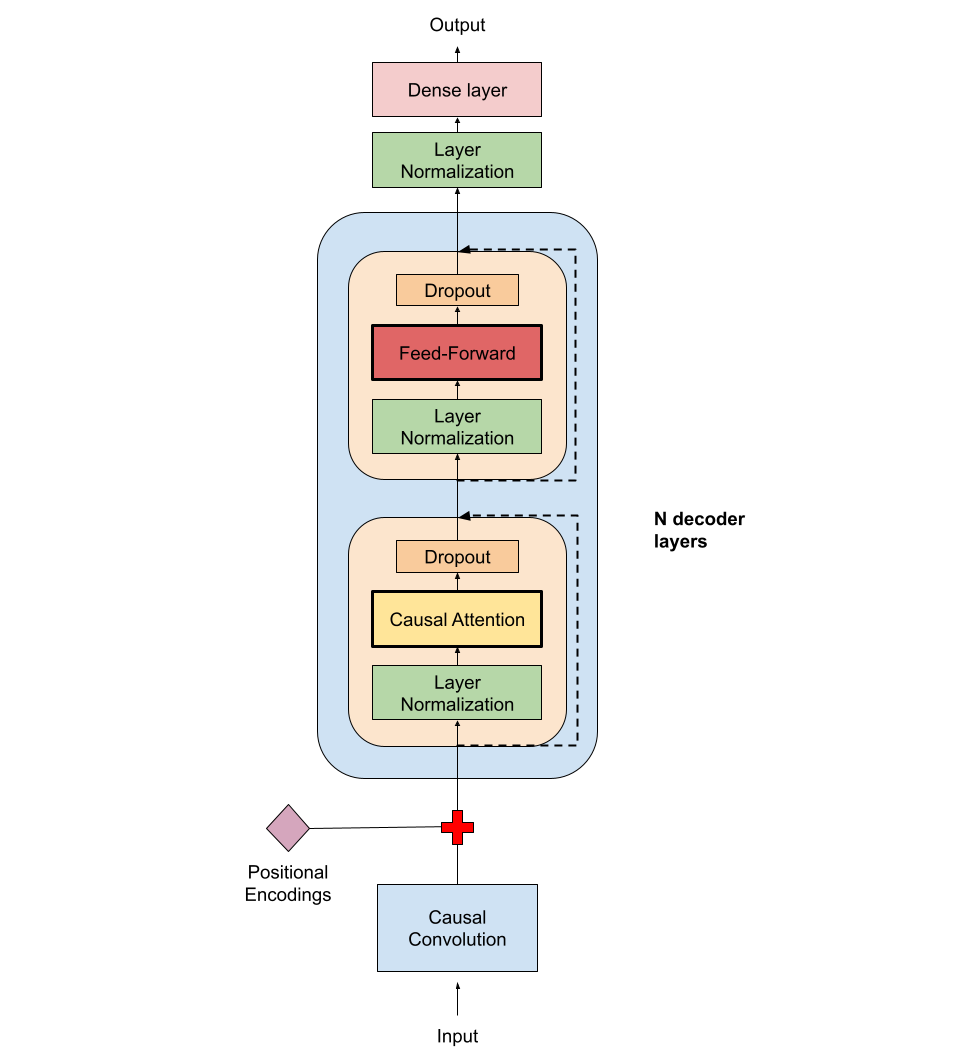
\includegraphics[height=130mm]{decoder3.png}
	\caption{Transformer's architecture. The dotted lines represent residual connections. \label{our-decoder}}
\end{figure}

%The Transformer in \cite{enhancing} is a modification of the original Transformer \pk{what is the original Transformer?} \cite{tr}, that uses only a decoder. \pk{what is a decoder?}
%We follow the same architecture type and therefore whenever we speak \pk{you don't speak} about the Transformer we will mean a decoder-only \cite{wikipedia} architecture one.

Our implementation of the Transformer model consists mainly of a causal convolution layer, positional encoding layer, $N$ identical decoder layers, layer normalization and a fully-connected layer. 
Most of the layers' outputs have $d_{model}$ dimension.
I present the general architecture on Figure ~\ref{our-decoder}.

\textbf{Positional encoding} allows us to feed the model embedded information about how the data points are ordered in the inputted time series.
We use a trainable embeddings for the positional encodings and add it to the input before it reaches the first decoder layer. \pk{???} \mn{I changed it a little, but I am not sure whether it is still confusing.}

A single \textbf{decoder} layer consists of a causal attention sub-layer and a feed-forward sub-layer:
\begin{itemize}
	\item The feed-forward sub-layer contains a simple feed-forward neural network with two dense layers and a ReLU activation in-between.
	\item The causal attention sub-layer contains the attention mechanism that I describe later on.
\end{itemize}

Both sub-layers are residual and wrapped with a layer normalization and a dropout layer.

\section{Attention}

\subsection{Scaled Dot-Product Attention}

Attention is the key part to explaining how the Transformer works.
It enables us to train the neural network to encode the relations between different parts of the input (e.g., a time series' data points).


%It allows us to train an approximated dictionary which encodes the relations between different parts of the input.
%
%One needs to provide three matrices to the attention layer: keys, queries and values. They are all created from the input in a way that depends on the attention function.

Scaled dot-product attention introduced along with the Transformer architecture in \cite{tr} is perhaps the most known kind of attention function.
To calculate the attention score vector between one data point and all that come after, one first needs to provide a query vector for the first data point and a set of vector pairs consisting of keys and values for all the other data points. We match our query against all of the keys by a dot product and use the softmax function to normalize the result. Finally, by multiplying the softmax results with the corresponding values we get a set of weighted values vectors. After summing them we get the attention score vector for one data point.

One can informally see these calculations as operations on a neural network-approximated dictionary, where each key corresponds to a certain value and we treat the dot operation between the query and keys as a measure of similarity. When they are orthogonal, the dot product will be equal to 0. On the other hand, for vectors of fixed length the dot product is maximal when they have the same direction. When the result of softmax is large between two data points, we can informally say that the attention relates these two points.
\newline

In reality we do not need to calculate the attention sequentially for every data point, but rather use matrix operations.
One needs to provide three matrices to the attention layer: $Q, K \in \mathbb{R}^{d_I \times d_k}, V \in \mathbb{R}^{d_I \times d_v}$ (respectively called queries, keys and values). They are created by multiplying the input matrix $I \in \mathbb{R}^{d_I \times d_{model}}$ with three distinct trainable weight matrices $W_Q \in \mathbb{R}^{d_{model} \times d_k}, W_K \in \mathbb{R}^{d_{model} \times d_k}, W_V \in \mathbb{R}^{d_{model} \times d_v}$.

For given $Q, K, V$ we compute the attention with the following formula:

$$ Attention(Q, K, V) = softmax(\frac{QK^{T}}{\sqrt{d_k}} \cdot M)V \textrm{ (from \cite{enhancing})} $$

\pk{a picture is worth a thousand words} \mn{I think here maybe it's worth adding some words, since I did not talk a lot about the informal understanding of attention. Above I added some paragraphs about how to calculate and understand it. If I were to add a picture, maybe the one from the paper (Figure 2 in Attention...)? But I think this formula is very short anyways.}

where $d_k$ stands for the dimension of $Q$ and $K$. Dividing by its square root is supposed to balance out the growth of $Q$ and $K^{T}$ dot product that occurs with larger values of $d_k$.

$M$ is a \textbf{mask matrix} that sets all the elements corresponding to connections between future and past (upper triangular) to $-\infty$. It prevents the model from attempting to relate the past events to the future ones. \pk{show the matrix} \mn{I fixed it right now, since I see I was wrong before of how it should look like. Not sure whether you'd still want me to show it, since it should be one of the simplest matrices spoken about here. WDYT?}


%One might informally understand the attention as a way to train a neural network dictionary, where 


While calculating the softmax score for any two data points in a time series, the scaled dot-product attention does not use any information about other data points. We call this property \textbf{context-blindness}. Sometimes this might lead the model to assigning strong attention score between events that have similar values, even if their contexts (neighboring data points) are very different. That might cause the model to incorrectly recognize patterns in the time series (\cite{enhancing}).

\subsection{Convolutional Attention}

%\subsection{Causal convolution} \pk{what is convolution? a good place for some pictures}
\begin{defi}\label{ts}
	\textbf{Causal convolution} is a convolution used on input padded with $k - 1$ zeros at the start, where $k$ denotes the size of the kernel.
	
\end{defi}
%
This type of convolution is particularly useful for time series, since it enables us to make predictions with only partial input, essentially generating a completely new time series.
\newline

The convolutional attention \cite{enhancing} is calculated in almost the same way as the scaled dot-product attention. 
It only differs in the way it computes queries and keys.
Instead of applying a matrix multiplication with weight matrices, it uses a causal convolution with a stride of 1. When the kernel's size is equal to 1 it is equal to the matrix multiplication.

The usage of convolution is supposed to offset the dot-product attention's context-blindness. Since the convolution layer learns to recognize input's context, stronger attention score should be assigned to similar events.

\subsection{Multi-headed attention}

Each attention block might contain more than one parallel attention layer, aka attention "head". In theory this allows for different layers to learn various kinds of relationships in the input and is a very successful tool e.g. in natural language processing \cite{tr}.

The outputs of all $h$ attention heads are concatenated and multiplied by a weight matrix $W^O \in \mathbb{R}^{hd_{v} \times d_{model}}$ to squeeze them back into $d_I \times d_{model}$ shape before passing them to the next layer.

To offset the additional computational cost related with multiple attention heads, we set $d_k$ and $d_v$ to $d_{model} / h$.

\section{Training}

\subsection{Additional input} \pk{what is a covariate?} \mn{I changed the name since it's not really necessary to call these covariates.}

Following \cite{enhancing}, we use additional variables as part of the model's input aside the time series itself.
There are three kinds of additional input we use:
\begin{enumerate}
	\item Numerical information about time the input was recorded (year, month, day-of-the-week, hour-of-the-day, minute-of-the-hour). 
	%We normalize them and store in one dimension.
	\item Identifier of the time series.
	%Embedded identifier of the time series with the same dimensionality as positional embeddings.
	\item Input's distance from the sequence's start. 
	%We normalize them in the same way as the time input.
\end{enumerate}
We embed all of the additional variables to the same dimension, sum those embeddings and normalize them. Finally, we add the result to our model's (embedded) input and normalize it as well.
%The input to our model consists of normalized summation of the 
% summed identifier embeddings and positional embeddings concatenated with rest of the additional variables and the time series itself.

%\subsection{Scale handling}

\subsection{Weighted sampling}

We adapt a weighted sampling technique in our training, similarly to \cite{enhancing} and \cite{deepar}. Its main purpose is to counteract model's tendency to underfit data of a large scale, since it occurs more rarely in the datasets. We test that idea by including the weighted versus uniform sampling in our grid searches.

We calculate the weights by normalizing the scale factor $v_i$:

$$ v_i = 1 + \frac{\sum^{T}_{t=1} y^{(i)}_t}{T} \text{,}$$
where $T$ is $y^{(i)}$'s length.

\section{Metrics}

\subsection{Quantile loss}

Quantile loss is a metric designed to evaluate and/or train models designed with quantile prediction in mind.
We define $\rho$-quantile loss as follows:

$$ QL_\rho(\hat{y}, y) = max(\rho(y - \hat{y}), (\rho - 1)(y - \hat{y})) \text{,} $$

\pk{picture maybe?} \mn{I would do something like here: https://towardsdatascience.com/quantile-regression-from-linear-models-to-trees-to-deep-learning-af3738b527c3 or (best) borrow it, but I am not sure how it works with licenses and copyrights?}

where $\hat{y}$ denotes the model's prediction for the $\rho$ quantile and $y$ is the ground truth value.

This metric is characterized by a stronger penalization of over-predictions for $\rho$ smaller than 0.5, and under-predictions for $\rho$ greater than 0.5. \pk{good intuition}

\subsection{Risk metric}

$Risk_\rho$ is a type of normalized quantile loss metric defined as follows for $\rho \in (0,1)$:

$$ Risk_\rho(\hat{\textbf{y}}, \textbf{y}) 
= 2\frac{\sum_{i,t}QL_\rho(\hat{y}^{(i)}_t, y^{(i)}_t)}
{\sum_{i,t} |y^{(i)}_t|}$$

%, where $y^{(i)}_t$ denotes $t$ time step of a series number $i$.

It is very popular in time series prediction papers that use the Transformer (e.g. in \cite{enhancing}, \cite{deepar}), which lead us to choose it as the metric we use in the model's evaluation. \pk{sure, but why use it specifically in our case, over pointwise metrics?} \mn{I added some details here:} Furthermore, quantile loss allows us to assess how well our model estimates series' extreme values. It is useful for applications like electricity consumption risk estimation, where one might ask how likely it is in the given time-frame that the power consumption reaches a certain level. 

%\begin{defi}
%	$\rho$-quantile loss
%\end{defi}

%We define $\rho$-quantile loss for $\rho \in (0,1)$ as follows:
%
%$$ R_\rho(x, ) $$

%\begin{defi}
%	\textbf{The encoder} is a stack of identical layers. Each layer has two sub-layers.
%\end{defi}
%We use a standard "scaled dot-product attention"\cite{tr}.
%We can define self-attention as a function that takes as an input a query and 


% Causal convolution: https://github.com/christianversloot/machine-learning-articles/blob/main/how-to-use-padding-with-keras.md

\chapter{Approximating a continuous distribution with the Transformer}



% serializacja inputu (a nie outputu):
% omijamy problem skalowania inputu
% czy weighted sampling jest uzyteczne dla serial?
% napisz ze mozna meaningful embeddings dac do zserializowanego inputu.

While the Transformer was already proved to be a very efficient tool for the time series prediction, we believe it has a lot more potential that could be used without changing its architecture.
%can be utilized even better for this purpose. 
Previously neural networks including the Transformer were commonly used for predicting parameters of a simple distribution like Gaussian for each forecasted point in time (\cite{deepar}, \cite{enhancing}). In this work we would like to expand that idea to modeling any continuous distribution by approximating it with a categorical one.
%Although the most common idea is to use the neural network for predicting a simple distribution l
%We anticipate that the Transformer does not need the common simplification of the time series forecasting task to the Gaussian's parameters prediction like the one used in \cite{enhancing}.
 %Specifically, one can apply it to model (almost) any distribution using the fact that one can approximate a continuous distribution using a categorical one. 
This is made possible by leveraging Transformer's success in tasks requiring prediction of thousands categories like language translation. 
%Since one can approximate a continuous distribution using a categorical one, it might be an actually more sustainable and efficient approach than the one from \cite{enhancing}.
%We anticipate that the Transformer does not need the usual simplification of the time series forecasting task to the Gaussian's parameters prediction.

This thesis explores whether the Transformer's performance on time series prediction can be improved by training it to predict a categorical distribution for each point in the sequence instead of a Gaussian distribution. Later on we directly compare both approaches.
%Furthermore, by using the same serialization process for the input we hope to 

\section{Serialization}

We call \textbf{serialization} the reversible process of bucketing each value in a real-valued series, i.e. mapping it to a discrete category from a finite number of categories.
We hypothesize that serializing and embedding the time series before feeding it to a Transformer can make it easier for the model to train.

The reverse process is named \textbf{deserialization} and it can be used for approximating a continuous distribution with a categorical one.

%Our serialization algorithm requires two parameters: maximum value we expect in the datasets (\textbf{high}), minimal (usually equal to 0) and exact number of categories (\textbf{vocabulary_size}).
Our serialization algorithm requires two parameters: maximum value we expect in the datasets ($high$), minimal (usually equal to 0) and the exact number of categories ($vocabulary\_size$).
We simply spread the categories uniformly from the minimal value to the maximal one. 

Deserialization is the reverse of this process in which we output the minimal value assigned to a specific bucket. Since the number of categories we use is finite, serialization is bound to lose the precise value of some data points in a series. With enough buckets used, we expect this drop in precision should be negligible in comparison to our gains in the prediction's reliability.

\section{Serial Predictor}
The main novelty of our work is a time series forecasting model named Serial Predictor.
We use the Transformer's architecture as described in Section~\ref{s:architecture}. Our input consists of serialized and embedded time series. The model outputs $vocabulary\_size$ logits, each of them corresponding to a single bucket. We use a category cross entropy loss to train our model.


% Analiza tego że to dobrze powinno działać kiedy jest risky sytuacja (nagła zmiana)

\chapter{Experiments}

In our experiments we decided to compare our Serial Predictor with a time series forecasting model that we call Gaussian Predictor. This model uses the same Transformer body as Serial Predictor, but it does not use the serialization on its input and outputs parameters of a Gaussian distribution. We use logistic loss for training the Gaussian Predictor.
%This model is based on the one described in \cite{enhancing} and uses convolutional self attention 
%and uses the same Transformer body as the Serial Predictor, but it 

\section{Datasets}

I chose two datasets for presenting our results in this thesis: $electricity$ and $traffic$. They are both based on real-world data and are easily accessible through the GluonTS (\cite{gluonts}) package. Furthermore, they are used in many of the papers we base our work on (\cite{enhancing}, \cite{deepar}), which makes them a good reference point.

The $electricity$ dataset is the electric consumption data collected from 370 customers recorded with a frequency of 1 hour (\cite{enhancing}, \cite{deepar}). The $traffic$ dataset consists of the hourly occupancy rates of 963 lanes in San Francisco (\cite{enhancing}, \cite{deepar}). Since $traffic$ displays higher differences between patterns observed in weekends and weekdays, it is considered a more demanding dataset and is useful for finding out how well the model can capture both long-term and short-term dependencies (\cite{enhancing}).


\section{Noise analysis in the datasets}
%Tu opisz czemu uważamy że nie jest gaussowski, wykres jakiś twój + analiza Łukasza

In our preliminary analysis we decided to investigate whether 



\section{Differences from previous works}\label{s:diff}

During the late stages of our work we contacted the authors of \cite{enhancing} and received their code. We discovered that there was a significant difference in our evaluation processes. 
Mainly, the author's predictions of multiple time steps during the evaluation were always ran based on historical data points (not autoregressively). Our suspicion is that this effect was not the authors' intention and might lead to differences in the results, since it makes the task easier for the model.

Additionally, the datasets provided by GluonTS (\cite{gluonts}) are not identical to the ones used in the experiments from \cite{enhancing} or \cite{deepar}. Even though the data's source is the same, its processing was different (https://github.com/awslabs/gluon-ts/issues/830).

Furthermore, we did not include the sparse attention in our experiments. We also did not use the risk metric as the loss function, which might have impacted the model's performance negatively. All these differences should not have contributed to the gap between Gaussian and Serial Predictors, though. 


\section{Experiments setup}

We used the Adam optimizer for all our experiments along with a rsqrt decay learning rate scheduler.
Every experiment was run as follows:
\begin{itemize}
	\item We used $n\_steps = 1000000$ training steps, with $1000$ warm-up steps  ($warmup\_steps = 1000$) and $batch\_size = 16$.
	%\item We use $warmup\_steps = 1000$
	\item The evaluation was run every $eval\_every = 1000$ steps over $n\_eval\_batches = 128$ samples.
	\item Sampled sub-sequences' length was equal to $series\_length = 768$.
\end{itemize}
We ran a randomized parameter grid search over the following parameters:
\begin{itemize}
	\item Convolutional attention's kernel size: $conv\_attention\_kernel\_width \in \{ 1, 2, 3, 6, 9 \}$
	\item Number of heads in the multi-headed attention: $ n\_heads \in \{ 1, 2, 4 \} $
	\item Dropout rate (same in various places): $dropout \in \{ 0.1, 0.2, 0.3, 0.4, 0.5 \} $
	\item Most of the layers outputs' size: $d\_model \in \{ 64, 128, 256, 512 \} $
	\item Number of decoder layers: $n\_layers \in \{ 2, 4, 6 \}$
	\item Learning rate's scheduler constant: $multifactor.constant \in \{ 0.001, 0.003, 0.01, 0.03, 0.1 \}$
	\item Usage of weighted sampling: $weighted\_sampling \in \{ True, False \}$
	\item (Serial Predictor only) Maximum value we can predict: $high \in \{2, 5, 10\}$ 
	\item (Serial Predictor only) Number of buckets: $vocab\_size \in \{1024, 2048, 4096\}$ 
\end{itemize}

We ran every experiment with a 16GB of RAM limitation on the Entropy cluster (\cite{entropy}) containing various GPUs: GTX 1080 Ti, Titan X, Titan V, RTX 2080 Ti and RTX A6000.


Evaluations were carried out autoregressively over a prediction length of 24 hours.

% można opisać proces averagowania wyników, ale nie wydaje mi się to tak istotne.


\section{Results}

% powinnaś pokazać:
% - high
% - vocab size
% weighted sampling
% jeśli n_heads będzie ciekawe, to n_heads


\begin{table}[h]

\begin{center}
\begin{tabular}
	{ |p{2cm}|p{1.5cm}|p{1.5cm}||p{1.5cm}|p{1.5cm}||p{1.5cm}|p{1.5cm}|  }
	\hline
	& \multicolumn{2}{c||}{Gaussian Predictor} & \multicolumn{2}{|c||}{Serial Predictor} & \multicolumn{2}{|c|}{Enhancing Locality (\cite{enhancing})} \\
	\hline
	& \hfil $R_{0.5}$ & \hfil $R_{0.9}$ & \hfil $R_{0.5}$ & \hfil $R_{0.9}$
	& \hfil $R_{0.5}$ & \hfil $R_{0.9}$
	 \\
	 
	 
	\hline
	electricity & \hfil 0.127   & \hfil 0.087    & \hfil 0.069 &   \hfil 0.052 & \hfil 0.070 & \hfil 0.044 \\
	traffic &  \hfil 0.402   & \hfil 0.224   & \hfil 0.135 &   \hfil 0.101 & \hfil 0.139 & \hfil 0.094\\
	\hline
\end{tabular}
\caption{\label{tab:results}Results of our best performing models' and the ones cited from $\cite{enhancing}$. The best results for each dataset and metric are marked in bold.}
\end{center}
\end{table}

% TODO: do the bold

% różnice w datasetach i ich stopniu trudności omówić
% brak reproducibility 
% 



%\begin{center}
%	
%	\begin{tabular}{ p{2cm}p{1.5cm}p{1.5cm}p{1.5cm}p{1.5cm}  }
%
%		& \multicolumn{2}{c}{Gaussian Predictor} & \multicolumn{2}{c}{Serial Predictor} \\
%%		\hline
%		& \hfil $R_{0.5}$ & \hfil $R_{0.9}$ & \hfil $R_{0.5}$ & \hfil $R_{0.9}$ \\
%		\hline
%		electricity & \hfil 0.127   & \hfil 0.087    & \hfil 0.069 &   \hfil 0.052 \\
%		traffic &  \hfil 0.402   & \hfil 0.224   & \hfil 0.135 &   \hfil 0.101\\
%		\hline
%	\end{tabular}
%	
%\end{center}

We have not managed to reproduce the results from $\cite{enhancing}$ with our Gaussian Predictor, which we attribute to many differences in our work that we investigated as I described in the section \ref{s:diff}. There is, however, a large gap between the performance of our Gaussian Predictor and the Serial one in every evaluated metric and dataset, with the Serial Predictor scoring almost a third of the $R_{0.5}$ metric over the $traffic$ dataset. Furthermore, the Serial Predictor performs better in some categories from the model cited from $\cite{enhancing}$ despite the differences that we found out in the late study stages that were unfavorable for our evaluation process.


%suggesting that further work on searching for a good baseline and evaluation methods 

% Additionally, the datasets provided by \cite{gluonts} are not identical to the ones 

% różnica w datasetach!11111111



\chapter{Conclusion}

\section{Summary}

This thesis compares the accuracy of a Transformer model architecture used for the time series prediction in two ways. The first one is based on important past time series works and involves using the Transformer to predict the parameters of a Gaussian distribution for each forecasted time point. The second way is our Serial Predictor that approximates a continuous distribution with a categorical one. The early results of our work are very promising but also suggest a need to search for a good reproducible baseline reference in the future research.

\section{Further work}

While the work presented in this thesis uses its own fair baseline model, the further experiments should focus on reproducing or readjusting the results from \cite{enhancing} and crafting a consistent comparison with the past time series research.

Furthermore, it is important to attempt finding datasets that might benefit even more from our approach in comparison to established Transformer-based time series models. Since the Serial Predictor can theoretically be trained to output almost any distribution, we hope that it might perform better on data that has low determinism qualities like the stock or cryptocurrency markets.

This work also suggests that it might be beneficial for any further research applying the Transformer model to try leveraging its ability to successfully predict many categories.
This is especially relevant in fields where previous works simplified a task to one where it is easier to apply less complicated, non-neural network approaches.


\begin{thebibliography}{99}
\addcontentsline{toc}{chapter}{Bibliography}

%\bibliography{bibFile}


%@article{einstein,
%	author =       "Albert Einstein",
%	title =        "On the electrodynamics of moving bodies",
%	journal =      "Annalen der Physik",
%	volume =       "322",
%	number =       "10",
%	pages =        "891--921",
%	year =         "1905"
%}
%
\bibitem{enhancing} Shiyang Li, Xiaoyong Jin, Yao Xuan, Xiyou Zhou, Wenhu Chen, Yu-Xiang Wang and Xifeng Yan. \textit{Enhancing the Locality and Breaking the Memory
	Bottleneck of Transformer on Time Series Forecasting}. arXiv:1907.00235, 2019.

\bibitem{lstm} Sepp Hochreiter and Jürgen Schmidhuber. \textit{Long short-term memory}. Neural computation, 9(8):1735–1780, 1997.

\bibitem{gru} Kyunghyun Cho, Bart Van Merriënboer, Dzmitry Bahdanau, and Yoshua Bengio. \textit{On the properties of neural machine translation: Encoder-decoder approaches}. arXiv preprint arXiv:1409.1259, 2014.

\bibitem{context} Urvashi Khandelwal, He He, Peng Qi, and Dan Jurafsky. \textit{Sharp nearby, fuzzy far away: How neural language models use context}. arXiv preprint arXiv:1805.04623, 2018.

\bibitem{tr} Ashish Vaswani, Noam Shazeer, Niki Parmar, Jakob Uszkoreit, Llion Jones, Aidan N Gomez, Łukasz
Kaiser, and Illia Polosukhin. \textit{Attention is all you need}. NIPS 2017.

\bibitem{wikipedia} Peter J Liu, Mohammad Saleh, Etienne Pot, Ben Goodrich, Ryan Sepassi, Lukasz Kaiser, and Noam
Shazeer. \textit{Generating wikipedia by summarizing long sequences}. arXiv preprint arXiv:1801.10198, 2018.

\bibitem{deepar} Valentin Flunkert, David Salinas, and Jan Gasthaus. \textit{Deepar: Probabilistic forecasting with autoregressive recurrent networks}. arXiv preprint arXiv:1704.04110, 2017.

\bibitem{arima} George EP Box and Gwilym M Jenkins. \textit{Some recent advances in forecasting and control}. Journal of the
Royal Statistical Society. Series C (Applied Statistics), 17(2):91–109, 1968.

\bibitem{ssm} R. Hyndman, A. B. Koehler, J. K. Ord, and R .D. Snyder. \textit{Forecasting with Exponential Smoothing: The State Space Approach}. Springer Series in Statistics. Springer, 2008. ISBN
9783540719182

\bibitem{uber} Nikolay Laptev, Jason Yosinski, Li Erran Li and Slawek Smyl. \textit{Time-series extreme event forecasting with neural networks at Uber}. International Conference on Machine Learning.

\bibitem{stock1} J. L. Ticknor. \textit{A bayesian regularized artificial neural network for stock market forecasting}. Expert Systems with Applications, 40(14):5501–5506, 2013.

\bibitem{graph-forecast} Hongjie Chen, Ryan A. Rossi, Kanak Mahadik, Sungchul Kim and Hoda Eldardiry. \textit{Graph Deep Factors for Forecasting}. arXiv:2010.07373.

\bibitem{gluonts} Alexander Alexandrov, Konstantinos Benidis, Michael Bohlke-Schneider, Valentin Flunkert, Jan Gasthaus, Tim Januschowski, Danielle C. Maddix, Syama Rangapuram, David Salinas, Jasper Schulz, Lorenzo Stella,
Ali Caner Türkmen and Yuyang Wang. \textit{GluonTS: Probabilistic and Neural Time Series Modeling in Python}. Journal of Machine Learning Research.

\bibitem{entropy} https://entropy-doc.mimuw.edu.pl.

%\bibitem[Blar16]{eb1} Elizjusz Blarbarucki, \textit{O pewnych
%    aspektach pewnych aspektów}, Astrolog Polski, Zeszyt 16, Warszawa
%  1916.
%
%\bibitem[Fif00]{ffgg} Filigran Fifak, Gizbert Gryzogrzechotalski,
%  \textit{O blabalii fetorycznej}, Materiały Konferencji Euroblabal
%  2000.
%
%\bibitem[Fif01]{ff-sr} Filigran Fifak, \textit{O fetorach
%    $\sigma$-$\rho$}, Acta Fetorica, 2001.
%
%\bibitem[Głomb04]{grglo} Gryzybór Głombaski, \textit{Parazytonikacja
%    blabiczna fetorów --- nowa teoria wszystkiego}, Warszawa 1904.
%
%\bibitem[Hopp96]{hopp} Claude Hopper, \textit{On some $\Pi$-hedral
%    surfaces in quasi-quasi space}, Omnius University Press, 1996.
%
%\bibitem[Leuk00]{leuk} Lechoslav Leukocyt, \textit{Oval mappings ab ovo},
%  Materiały Białostockiej Konferencji Hodowców Drobiu, 2000.
%
%\bibitem[Rozk93]{JR} Josip A.~Rozkosza, \textit{O pewnych własnościach
%    pewnych funkcji}, Północnopomorski Dziennik Matematyczny 63491
%  (1993).
%
%\bibitem[Spy59]{spyrpt} Mrowclaw Spyrpt, \textit{A matrix is a matrix
%    is a matrix}, Mat. Zburp., 91 (1959) 28--35.
%
%\bibitem[Sri64]{srinis} Rajagopalachari Sriniswamiramanathan,
%  \textit{Some expansions on the Flausgloten Theorem on locally
%    congested lutches}, J. Math.  Soc., North Bombay, 13 (1964) 72--6.
%
%\bibitem[Whi25]{russell} Alfred N. Whitehead, Bertrand Russell,
%  \textit{Principia Mathematica}, Cambridge University Press, 1925.
%
%\bibitem[Zen69]{heu} Zenon Zenon, \textit{Użyteczne heurystyki
%    w~blabalizie}, Młody Technik, nr~11, 1969.

\end{thebibliography}

\end{document}


%%% Local Variables:
%%% mode: latex
%%% TeX-master: t
%%% coding: latin-2
%%% End:
